\clearpage
\section{Theoretische Grundlagen}
\subsection{Radioaktive Zerfälle}
Instabile Kerne können unter Aussendung charakteristischer radioaktiver Strahlung zerfallen. Dieser Zerfall kann auf unterschiedlichen Wegen geschehen und dabei können unterschiedliche Arten von Strahlung frei gesetzt werden. Radioaktiver Zerfall ist ein statistischer Prozess, dabei ist die Änderung einer radioaktiven Probe $dN$ nach einer Zeit $t$ proportional zur gesamten Menge der Probe N:
\begin{center}
\[\frac{dN}{dt}=-\lambda N \]
\end{center}
Eine Lösung zu dieser Differentialgleichung erhält man durch separieren der Variablen und erhält durch integrieren:
\begin{center}
\[\ln N(t)-\ln N(0)= \int\limits_{N(t)}^{N(0)}\frac{dN'}{N'}=- \int\limits_{t}^{0}\lambda dt'= -\lambda t \]
\[ \Leftrightarrow \ln{\frac{N(t)}{N(0)}} = -\lambda t\]\\
\[ \Leftrightarrow N(t)= N(0) \exp(-\lambda t)\]
\end{center}
Aus dieser Formel lässt sich nun auch die Halbwertszeit $T_{\frac{1}{2}}$ berechnen:
\begin{center}
\[ \frac{1}{2}N_0 = N(T_{\frac{1}{2}}) = N_0 \exp(-\lambda T_{\frac{1}{2}})\]\\
\[ \Leftrightarrow T_{\frac{1}{2}} = \frac{\ln 2}{\lambda}\]
\end{center}
Und für die Lebensdauer gilt
\begin{center}
\[ \tau = \frac{1}{\lambda}= \frac{T_{\frac{1}{2}}}{\ln 2}~~. \]
\end{center}

\subsubsection{$\alpha$-Strahlung}
Bei dieser Strahlung zerfällt der Mutterkern $^{A}_{Z}X$ mit Massenzahl A (Anzahl an Protonen und Neutronen im Kern) und Kernladungszahl Z (Anzahl Protonen im Kern) unter Aussendung eines zweifach positiv geladenen Heliumkerns $^{4}_{2}He^{2+}$ zu dem zweifach negativ geladenen Tochterkern $^{A-4}_{Z-2}Y^{2-}$, wobei Energie frei wird, wie folgender Gleichung entnommen werden kann: \[^{A}_{Z}X\rightarrow ^{A-4}_{Z-2}Y^{2-}+^{4}_{2}He^{2+}+\Delta E\]
Die freiwerdende Energie hängt von den Reaktionskernen ab und ist diskret. Typischerweise hat die $\alpha$-Strahlung eine Energie im Bereich einiger MeV. Da die ausgesandten $^{4}_{2}He^{2+}$-Kerne elektrisch geladen und ziemlich schwer sind, ist die Reichweite dieser Strahlung sehr gering (in Luft wenige cm). Bereits ein Blatt Papier reicht aus, um $\alpha$-Strahlung abschirmen zu können.
\subsubsection{$\beta$-Zerfall}
Es gibt drei verschiedene Arten von $\beta$-Zerfall: $\beta^+$- und $\beta^-$-Zerfall und den Elektroneneinfang (EC, Electron Capture).\\
~\\
\textbf{$\beta^+$-Zerfall:} Bei Kernen mit relativem Überschuss an Protonen kann $\beta^+$-Zerfall auftreten. Dabei wird ein Proton unter Aussendung eines Positrons und eines Neutrinos in ein Neutron umwandelt:
\begin{center}
$\mathit{_1^1p \rightarrow _0^1n + e^+ + \nu}$
\end{center}
Die Kernladung verringert sich um eins. Das Positron wird sich nach seiner Abbremsung durch Materie bald mit einem Elektron zu einem Positronium-Atom vereinigen, welches nach einer mittleren Lebensdauer von $10^{-7}$s bis $10^{-9}$s in zwei $\gamma$-Quanten zu je 511keV zerfällt.\\
~\\
\textbf{$\beta^-$-Zerfall}: Bei Kernen mit relativem Überschuss an Neutronen kann $\beta^-$-Zerfall auftreten. Hierbei wandelt sich ein Neutron in ein Proton um, unter Aussendung eines Elektrons und eines Antineutrinos, welches ein Teil der Zerfallsenergie weg trägt:
\begin{center}
$\mathit{_0^1n \rightarrow _1^1p+e^- + \overline{\nu}}$
\end{center}
Die Kernladung verringert sich um eins. Die Energie der ausgesendeten Elektronen ist kontinuierlich verteilt.\\
~\\
\textbf{Elektroneneinfang (EC, Electron Capture)}: Vor allem bei schweren Kernen mit Protonenüberschuss tritt EC auf. bei diesem Effekt wird ein Elektron aus der K-Schale vom Kern eingefangen unter Aussendung eines Neutrinos, wodurch sich die Kernladungszahl um eins verringert. Der dadurch entstandene freie Platz in der K-Schale wird durch ein Elektron aus der, meistens nächst höheren L-Schale wieder aufgefüllt. Die durch den Übergang des Elektrons in die niedrigere Schale frei werdende Energiedifferenz wird als Röntgen- oder Augerstrahlung abgestrahlt. Der freie Platz in der L-Schale wird wiederum durch ein Elektron aus einer höheren Schale besetzt. Dieser Prozess setzt sich in Richtung äußerer Schalen fort bis eine stabile Elektronenkonfiguration wieder erreicht ist. Bei diesem Vorgang wird bei jedem Elektronenübergang eine für die entsprechende Energiedifferenz charakteristische Röntgenstrahlung frei gesetzt.\\
~\\
\textbf{Eigenschaften}: $\beta$-Strahlung hat im Gegensatz zu $\alpha$-Strahlung keine fest vorgegebene Energie, sondern ein kontinuierliches Spektrum an möglichen Energien, da die beim Zerfall frei werdende Energie auf den Atomkern, das Elektron/Positron und das Antineutrino/Neutrino verteilt wird. Dabei gibt es eine Maximalenergie, welche vom zerfallenden Kern abhängt. Typischerweise liegt diese in der Größenordnung von keV bis einigen MeV. Zur Abschirmung von $\beta$-Strahlung muss mindestens ein dünnes Blech verwendet werden. Die Reichweite von $\beta$-Strahlung in Luft beträgt einige Meter.
\subsubsection{$\gamma$-Strahlung}
Diese Art der radioaktiven Strahlung ändert weder die Massen-, noch die Ladungszahl eines Kerns. Sie beschreibt das Aussenden von elektromagnetischer Strahlung, wenn ein angeregter Kern in sein energetisches Grundniveau zurückfällt. Bei Zerfallsprozessen tritt die $\gamma$-Strahlung als Begleiterscheinung nach einem $\alpha$- bzw $\beta$-Zerfall auf. Da sie aus Photonen besteht, ist sie elektrisch neutral.
\subsection{Wechselwirkung von Photonen mit Materie}
Man nutzt die Wechselwirkung von $\gamma$-Quanten mit Materie um diese nachzuweisen. $\gamma$-Strahlen befolgen bei der Absorption folgendes Exponentialgesetz:
\begin{center}
$I_d=I_0e^{-\mu d}$
\end{center}
Wobei $I_0$ der Intensität vor dem absorbierenden Material entspricht, $I_d$ der Intensität bei einer Eindringtiefe $d$ und $\mu$ ist der Absorptionskoeffizient der absorbierenden Materie. Dieser Koeffizient hängt sowohl von $E_{\mu}$ als auch vom Absorber-Material ab.
Es gibt im Wesentlichen drei Wechselwirkungs-Mechanismen von $\gamma$-Quanten mit Materie deren Wirkungsquerschnitt mit der $\gamma$-Energie $E_{\gamma}$ und der Kernladungszahl $Z$ des Materials abhängt:
\subsubsection{Photoeffekt}
Der Photoeffekt tritt vor allem bei einer Energie $E_{\mu}$ < 200 keV (bei $Z \approx 50$) auf. Beim Photoeffekt überträgt ein $\gamma$-Quant seine Energie vollständig an ein Elektron, worauf dieses aus der Atomhülle geschlagen wird und erhält kinetische Energie. Die frei Stelle in der Atomhülle wird durch ein Elektron aus einer höheren Schale besetzt was zu den oben genannten Effekten führt.
\begin{figure}[h]
\begin{center}
\includegraphics[scale=0.3]{photoeffekt}
\caption{Schema zum Photoeffekt. Quelle: [onm]}
\label{fig:photo}
\end{center}
\end{figure}
\subsubsection{Comptoneffekt}
Der Comptoneffekt tritt überwiegend bei einer Energie von 200 keV < $E_{\gamma}$ < 5 MeV auf. Beim Comptoneffekt gibt ein $\gamma$-Quant beim Zusammenstoß mit einem Elektron nur ein Teil seiner Energie an das Elektron ab. Es wird an dem Elektron gestreut.

\begin{figure}[h]
\begin{center}
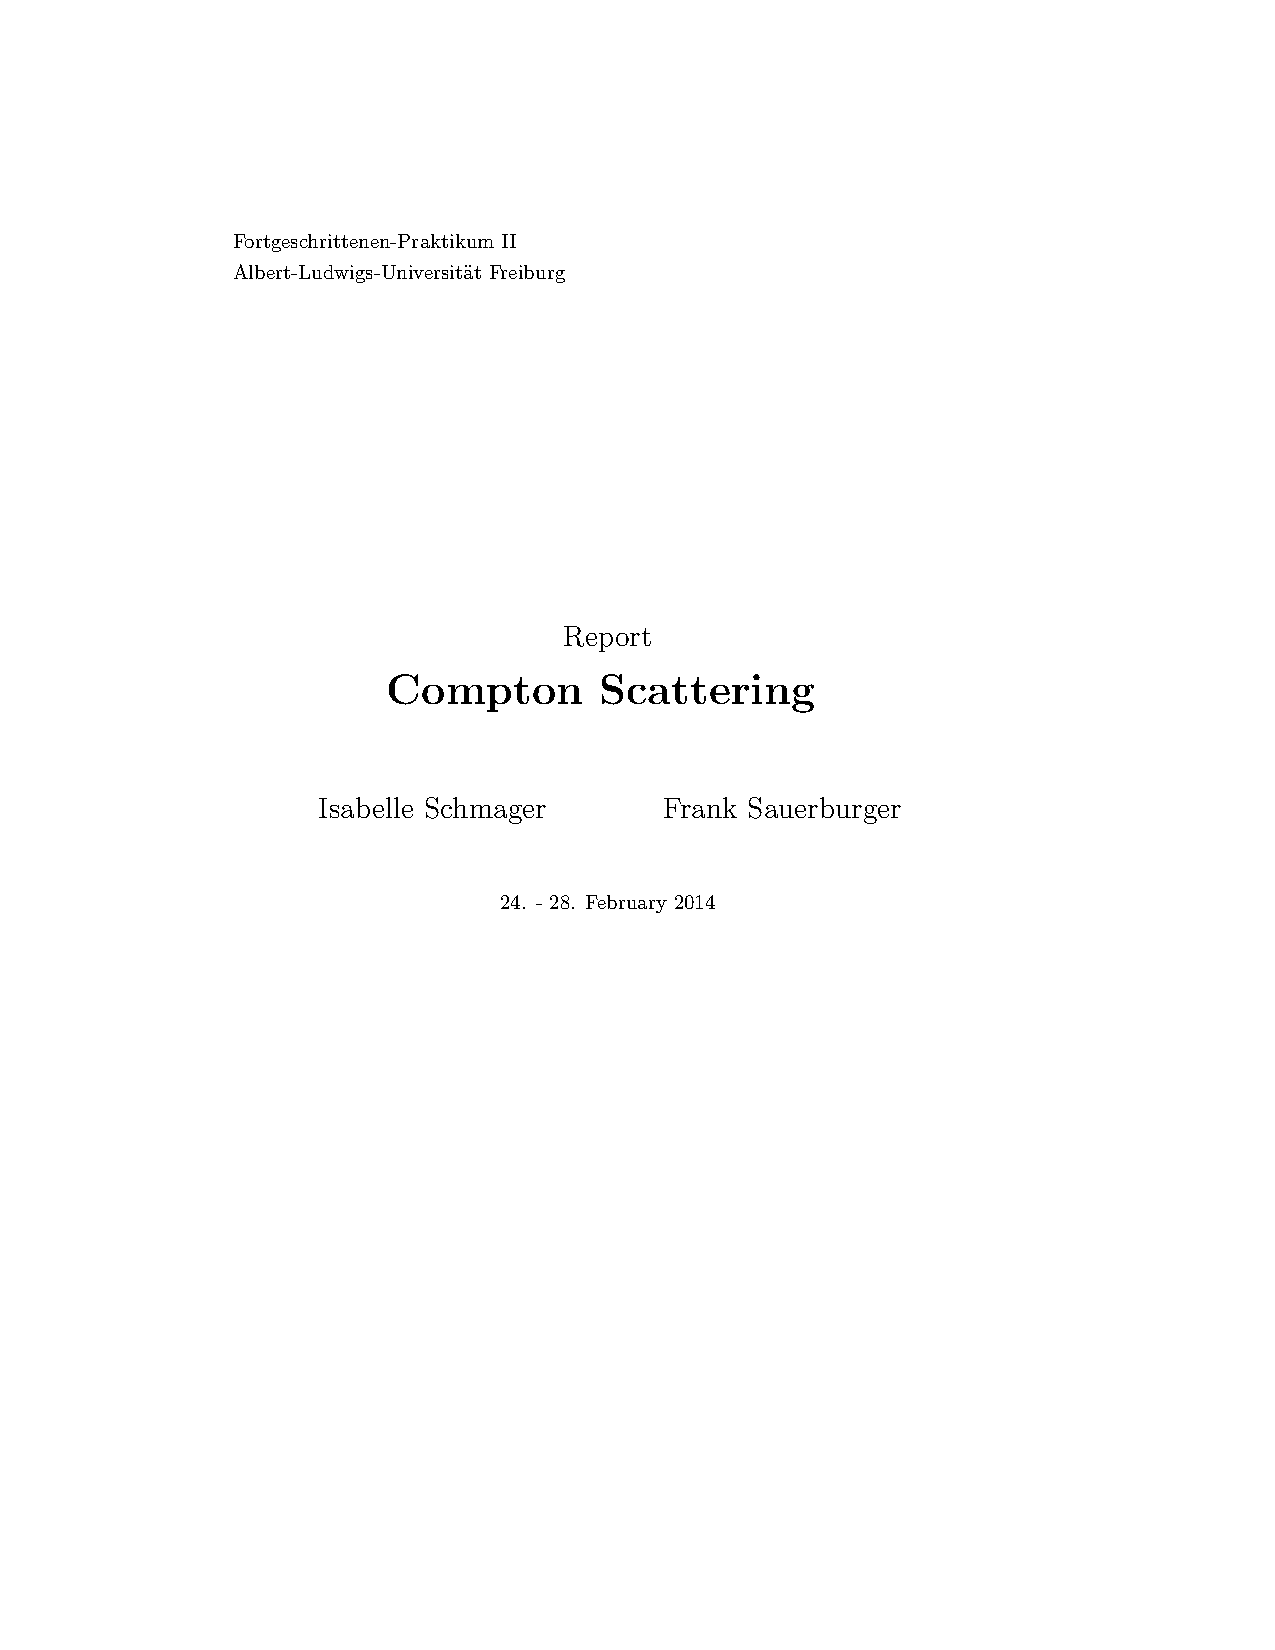
\includegraphics[scale=0.3]{compton}
\caption{Schema zum Comptoneffekt. Quelle: [ung]}
\label{fig:compton}
\end{center}
\end{figure}

\subsubsection{Paarbildung}
Paarbildung beobachtet man ab einer Energie $E_{\gamma} \ge$ 1,022 MeV. Paarbildung erhält man, wenn ein $\gamma$-Quant mit einem elektromagnetischen Feld eines Atomkerns oder eines Elektrons in Wechselwirkung tritt. Dabei wird das $\gamma$-Quant vollständig absorbiert und ein Positron-Elektron-Paar entsteht. Die Energie des $\gamma$-Quants wird auf die beiden Teilchen verteilt und der überschüssige Impuls wird vom Kern aufgenommen. Das Positron zerfällt zu zwei $\gamma$-Quanten mit je 0,511 MeV, da es nicht lange existieren kann und sich mit einem Elektron vereint.
\begin{figure}[h]
\begin{center}
\includegraphics[scale=0.3]{paarbildung}
\caption{Schema zum Paarbildung. Quelle: [onm]}
\label{fig:graph1}
\end{center}
\end{figure}
\subsection{Elektronik zum Nachweis vom $\gamma$-Quanten}
\subsubsection{Anorganischer Szintillator}
Das Prinzip der Detektion von Strahlung im Szintillator basiert auf dem Entstehen und Rekombinieren von Elektronen-Loch-Paaren. Trifft ein $\gamma$-Quant auf ein Elektron im Valenzband des Kristalls, so wird dieses in das Leitungsband gehoben und hinterlässt ein Loch. Nach einiger zeit fällt dieses wieder zurück in das tiefere Niveau unter spontaner Emission eines Photons. Dieses Photon hat jedoch genau die Energie mit der es wieder eine Elektron aus dem Valenzband in das Leitungsband hebt, welches seinerseits wieder ein Photon mit dieser Energie emittiert. Auf diese Weise können nur sehr wenige Photonen den Kristall verlassen, was in einem unmessbaren Signal resultiert. Um diesen Vorgang zu verhindern und die Lichtausbeute zu erhöhen, wird der Kristall dotiert, also mit Fremdatomen (Aktivtorzentren) versehen. Die zur Dotierung verwendeten Atome haben ein niedrigeres Leitungsband und stellen kleine Einbrüche im Leitungsband des Kristalls dar. Ein durch Strahlung angeregtes Elektron-Loch-Paar hat nun eine bestimmte freie Weglänge und wird, wenn es auf eine Vertiefung des Leitungsbandes trifft in diesem energieärmeren Zustand bleiben bis es rekombiniert. Das hierbei entstehende Photon hat nun eine kleinere Energie und gelangt aus dem Kristall heraus. Die messbaren Photonen eines Szintillationszählers haben Wellenlängen im sichtbaren oder UV-Spektrum. In unserem Versuch wurde ein Natriumiodidkristall verwendet.
\subsubsection{Organischer Szintillator}
Bei einem organischen Szintillator gibt es im Vergleich zum Anorganischen kein Leitungs- oder Valenzband. Einfallende $\gamma$-Strahlung regen die Moleküle des Detektormaterials an. Das Funktionsprinzip ist jedoch das gleiche wie beim anorganischen Szintillator. Die von den Aktivatormolekülen emittierten Photonen können nicht absorbiert werden und gelangen aus dem Szintillator heraus. Da jedoch die meisten durchsichtigen Materialien für UV-Strahlung nur eine geringe Reichweite haben muss ein zweites Material, eine so genannter Wellenlängenschieber dem Szintillator hinzugefügt werden. Dieses Material absorbiert höherfrequente Photonen und emittiert niederfrequente Photonen.\\~\\
Die Qualität eines Szintillator hängt im generell von der Lichtausbeute und der Auflösung von Energie und Zeit ab. Die verschiedenen Szintillatoren haben dabei verschiedene Vor- und Nachteile. Bei dem Natriumiodidkritsall erhält man eine sehr genaue Energieauflösung, jedoch ein sehr schlechte Zeitauflösung da dieser eine sehr lange Abregungszeit der Aktivatoratome aufweist. Beim Plastikszintillator hat man hingegen eine sehr gute Zeitauflösung aufgrund der kurzen Abregungszeit der Moleküle, die Energieauflösung ist dafür etwas kleiner.
\subsubsection{Photomultiplier}
Der Photomultiplier wandelt Lichtimpulse, in unserem Fall die vom Szintillator zugeleiteten, umzuwandeln in zur Lichtintensität proportionale elektrische Impulse umzuwandeln und diese durch Elektronenvervielfachung zu verstärken. Zum Umwandeln des der Lichtimpulse wird eine Photokathode benutzt. An ihr schlagen die ankommenden $\gamma$-Quanten, durch den Photoeffekt, Elektronen heraus. Ein $\gamma$-Quant kann mehrere Elektronen aus der Photokathode heraus schlagen welche durch eine anliegende Spannung zu ersten Dynode beschleunigt und befreien dort beim aufschlagen mehrere Sekundärelektronen, welche zur zweiten Dynode beschleunigt werden. Dies wiederholt sich bei allen weiteren Dynoden, da bei diesen sich jeweils die Spannung erhöht.

\begin{figure}[h]
\begin{center}
\includegraphics[scale=1.0]{PM}
\caption{Prinzipielle Funktionsweise eines Photomultipliers. Quelle: [hep].}
\label{fig:PM}
\end{center}
\end{figure}
